%% It is just an empty TeX file.
%% Write your code here.

\documentclass{article}

\usepackage{polyglossia}
\setmainlanguage{czech}

\usepackage[hidelinks]{hyperref}
\usepackage{xevlna}
\usepackage{xltxtra}
\usepackage{longtable}
\usepackage{pdflscape}
%\landscape otaci text ---- pdff landscape celou stranu na širku
\usepackage{graphicx}
\usepackage{biblatex}
\addbibresource{zdroje.bib}
%\usepackage{minted}
\usepackage{todonotes}



\title{Sazba v předmětu BI-DPR}
\author{Filip Novák}

\begin{document}
\maketitle

\tableofcontents
\listoftables
\listoffigures

\clearpage
%-------------------------------------------------------------------------------------------------------------
\section{Členění textu}

\subsection[Kapitoly]{Kapitoly, sekce podsekce}
Text členíme na kapitoly, (pod)sekce\dots{} Sekci vytvoříme příkazem
\textbackslash section\{\}
%-------------------------------------------------------------------------------------------------------------
\subsection{Odstavce}
Text --- zejména ten odborný --- je nutné členit na odstavce. Každý
odstavec by se měl týkat jednoho tématu, myšlenky \dots

Odstavce od sebe musí být vizuálně oddělené a různě vysázené. V
odborných textech je běžná sazba do bloku. Při ní je nutné vhodně měnit
mezislovní mezery. Jejich doporučená velikost je 0,25--0,33 čtverčíku.
%-------------------------------------------------------------------------------------------------------------
\section{Seznamy}
%-------------------------------------------------------------------------------------------------------------
\subsection{Odělování odstavců}

Běžně se používají dva styly:

\begin{description}
     \item[vertikální mezera] Dva odstavce jsou od sebe odděleny větší
meziřádkovou mezerou.
     \item[odsazení] První řádek odstavce je odsazený.
     \begin{itemize}
         \item Často se odsazení vynechává u prvního odstavce
     \end{itemize}
\end{description}
%-------------------------------------------------------------------------------------------------------------
\subsection{Jak vytvořit dokument v systému \LaTeX}
\begin{enumerate}
    \item Napište zdrojový soubor ve formátu \LaTeXe.
    \item Přeložte jej programem \verb|xelatex|.
\end{enumerate}
%-------------------------------------------------------------------------------------------------------------
\section{Tabulky} 
V tabulce \ref{tab:bodovane-cinnosti} najete možnosti, jak získat body v
předmětu BI-DPR\footnote{Dokumentace, prezentace, rétorika}.


    \begin{longtable}{p{3.5cm}|r|c}
    	\caption{Bodované činnosti v předmětu BI-DPR}
    	 \label{tab:bodovane-cinnosti}
    	\\
         činnost                    & body  & povinná \\ \hline \hline
         \endfirsthead
          činnost                    & body  & povinná \\ \hline \hline
         \endhead
        
         \multicolumn{3}{r}{\textit{Pokračován na další straně}} \\
         \endfoot
        
        \endlastfoot
         
         test citace                & 10    & ne \\ \hline
         test typografie            & 10    & ne \\ \hline
         hodnocení vedoucího        & 20    & ano \\ \hline
         test citace                & 10    & ne \\ \hline
         test typografie            & 10    & ne \\ \hline
         test typografie            & 10    & ne \\ \hline
         hodnocení vedoucího        & 20    & ano \\ \hline
         test citace                & 10    & ne \\ \hline
         test typografie            & 10    & ne \\ \hline
         hodnocení vedoucího        & 20    & ano \\ \hline
         obhajoba poziční zprávy    & 60    & ano \\ \hline
         
         
   
    \end{longtable}
    

\clearpage

\section{Samostatná práce} \label{sec:prace}
Ve zbytku času vysázejte ostatní části tohoto dokumentu --- samozřejmě
pomocí systému \LaTeX, doporučujeme \XeLaTeX.

\subsection{Prohlášení}
Prohlašuji, že jsem předloženoju práci vypracoval samostatně \dots{} bla
bla bla.

\subsection{Cíl}
Na řešení tohoto problému existují dva odlišné algoritmy:
\begin{enumerate}
    \item první,
    \item druhý.
\end{enumerate}

\noindent Clem \cite{guide} této práce je experimentální testování těchto vlastností:
\begin{itemize}
         \item zajímavá vlastnost,
         \item zajímavá vlastnost.
\end{itemize}

\section{Hodnocení}
Práce v sekci \ref{sec:prace} je nebodovaná. Další hodnocení ukazuje
tabulka \ref{}.
\begin{landscape}
\begin{table}[h!]\centering
\resizebox{1\textwidth}{!}{
    \begin{tabular}{c||c|c|p{5cm}}
         semestrální prácassdasdasdasdasde    asdasdasdasdasdasdasd      & body  & týmová    & popis \\
\hline \hline
         semestrální práce          & 0-100 & skupina   &  práce na celý
semestr, v některých pedmětech skupinová, v jiných individuální  \\
\hline
         úloha na progtest          &       & individuální
    \end{tabular}}
    \caption{Bodované činnosti v předmětu BI-DPR}
    \label{tab:bodovane-cinnosti}
    
\end{table}
\end{landscape}

\begin{landscape}
\begin{figure}
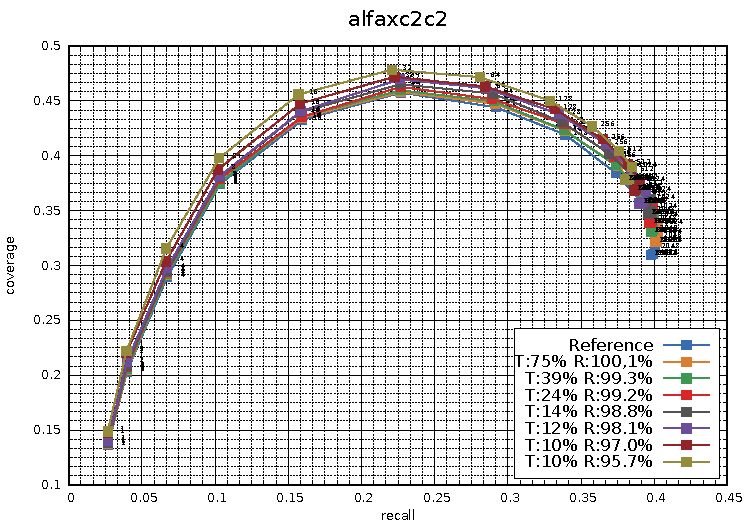
\includegraphics[width=1\textwidth]{1}
\caption{label}
\end{figure}
\end{landscape}


\section{TODO}
super. \todo{dopsat}


\section{Citace}
%\begin{thebibliography}{99}
%\bibitem{as}dome
%\end{thebibliography}
\printbibliography
\end{document}